
\documentclass[aps,prl,reprint]{revtex4-2}
\usepackage{gensymb}
\usepackage{graphicx}
\usepackage{amsmath}
\usepackage{hyperref}
\usepackage{dsfont}
\usepackage{relsize}
\usepackage{wrapfig}
\usepackage{graphicx}
\usepackage{hyperref}
\hypersetup{colorlinks=true, citecolor=blue, urlcolor=blue, linkcolor=blue}


\begin{document}

% Use the \preprint command to place your local institutional report
% number in the upper righthand corner of the title page in preprint mode.
% Multiple \preprint commands are allowed.
% Use the 'preprintnumbers' class option to override journal defaults
% to display numbers if necessary
%\preprint{}

%Title of paper
\title{FUEL Cell Lab}

% repeat the \author .. \affiliation  etc. as needed
% \email, \thanks, \homepage, \altaffiliation all apply to the current
% author. Explanatory text should go in the []'s, actual e-mail
% address or url should go in the {}'s for \email and \homepage.
% Please use the appropriate macro foreach each type of information

% \affiliation command applies to all authors since the last
% \affiliation command. The \affiliation command should follow the
% other information
% \affiliation can be followed by \email, \homepage, \thanks as well.
\author{Trevor Smith}
\email[]{smith.tr@northeastern.edu}
\homepage[]{https://github.com/trevorm4x/}
%\thanks{}
%\altaffiliation{}
\affiliation{Northeastern University}


\date{\today}

\begin{abstract}
	The efficiency of converting various forms of energy to and from 
	electrical energy were experimentally measured. The efficiency of a
	Silicon-based Solar Cell was found to be $15\ \pm\ 2\ \%$, in agreement
	with typical performance. The efficiency of an Electrolyzer was found to
	be $87\ \pm\ 6\ \%$, which is higher than typical performance. The 
	efficiency of a Hydrogen Fuel Cell was found to be $49\ \pm\ 5\ \%$,
	which is lower than typical performance. 
\end{abstract}


\maketitle

% body of paper here - Use proper section commands
% References should be done using the \cite, \ref, and \label commands
\section{Introduction}

Energy in various forms is of incredible relevance in the world today. Especially, electrical energy is the medium through
which most forms of energy are transmitted before being used. In this lab we explore the translation of energy from 
electromagnetic radiation, or light, to electrical energy, to chemical energy, and back to electrical energy.

A photovoltaic cell is a diode that forces any charge carriers freed by a photon hitting an electron through an electric 
circuit. Because of intrinsic properties of this problem efficiency is quite low, between fifteen and low-twenties percent.
An electrolyzer uses electricity to remove the bonds between hydrogen and oxygen in water, producing oxygen an hydrogen 
gas. Hydrogen gas is of particular relevance as the output, as oxygen is abundant in the atmosphere to react with the 
hydrogen. A hydrogen fuel cell does exactly this, essentially serving as a battery after separating the electrons and protons within hydrogen.

\section{Apparatus}

The apparatus consisted of the following.
\begin{itemize}
\item Hydrogen fuel cell apparatus, H-Tec, Model T-126
\item Optical Power Meter, Thorlabs, Model PM100-121C
\item 2 DVMs; decade resistor (1-100M$\Omega$)
\item Strong light source (flood light); 2.0V/ 2A power supply
\end{itemize}

\section{Efficiency of a Photovoltaic Cell}

\subsection{Procedure}

\begin{figure}[h]
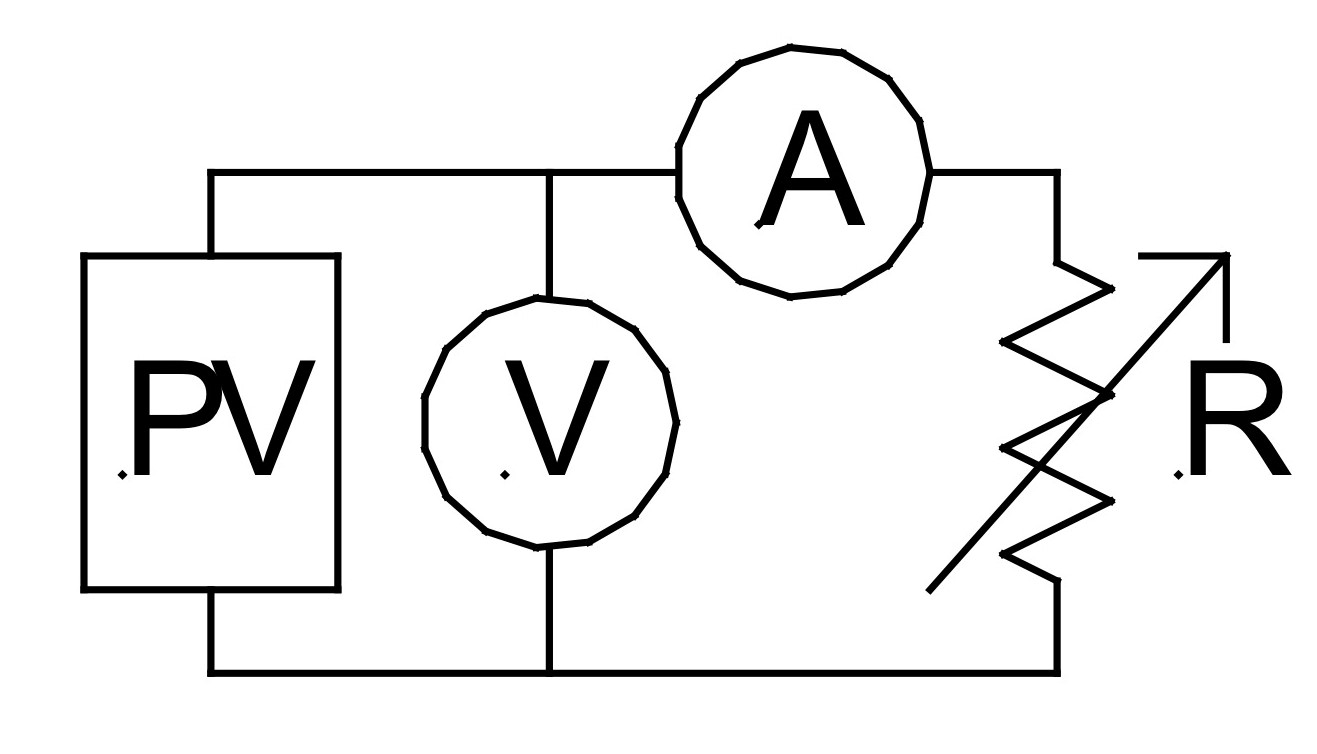
\includegraphics[width=0.4\textwidth]{../Images/l1_PartA.jpg}
\caption{\label{figA}Electrical circuit for measuring photovoltaic (PV) output voltage and current through a variable resistor (R). This curve reasonably matches theory.}
\end{figure}

A photovoltaic cell was used to power a simple circuit as given by \ref{figA},
while converting energy from a strong light source.
In order to measure the efficiency of the PV cell, the incident power in the 
form of light and the output power were both measured. 
A ThorLabs power meter was used to measure the intensity of the light at each 
individual PV cell, (intensity is given by power divided by area) and the
average intensity across the PV cell was multiplied by its measured area to 
find the power input to the system in the form of light. \\

In such a system, in order to measure the output power it is necessary to match
the resistance of the circuit to some unknown internal resistance of the PV cell. As such, a variable resistor was used to test various resistances in a 
logarithmic scale, and the peak output power was considered the optimal power
of the system.

\subsection{Results}

The intensity of light measured across the eight PV cells was found to be a
distribution of mean $28\ W/m^2$ and standard deviation $4\ W/m^2$. Multiplied 
by the area of the PV cells, the total light power hitting the PV cell was 
calculated at 0.22 Watts. \\

\begin{figure}[h]
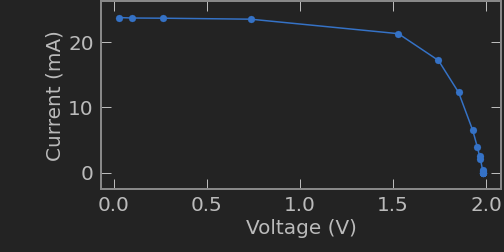
\includegraphics[width=0.45\textwidth]{../Images/l1_a_1.png}
\caption{\label{I(V)A}Current as a function of Voltage as resistance was varied.}
\end{figure}

\begin{figure}[h]
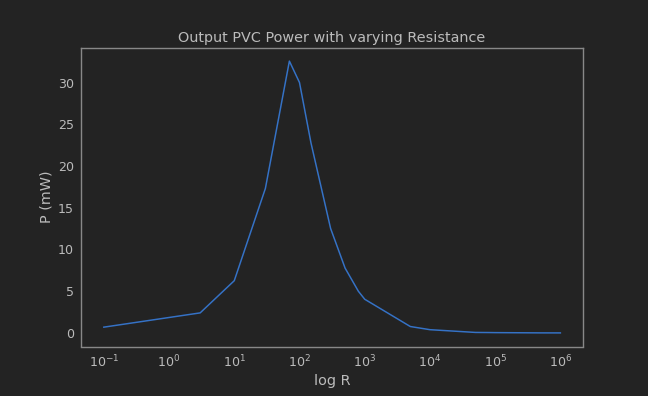
\includegraphics[width=0.45\textwidth]{../Images/l1_a_2.png}
\caption{\label{P(R)A}Power response of the circuit at various resistances.}
\end{figure}

The power response of the circuit was found to be a normal distribution when 
viewed on a logarithmic scale, with a maximum at 70 $\Omega$ and 32.5 mW. \\

\newpage
\begin{equation}
    \mathlarger{\eta_{PV}}=P_E/P_L
    \label{eta_PV}
\end{equation}
Where\ $\eta$\ is\ the\ efficiency\ of\ the\ fuel\ cell\ and\ P\ is\ Power.\\

Finally, the efficiency of the cell was computed by \ref{eta_PV} to be $15\ \pm\ 2\%$.

\subsection{Conclusions}
While there is a wide variety in efficiencies of PV Cells [\ref{Solar Cell}],
this falls somewhere inside it on the lower end. However, the significant 
uncertainty in this 
calculation is worth discussing. Primarily, this uncertainty stems from the 
wide distribution of light intensity hitting the cell at different points. In 
future verions of this experiment, more sophisticated models for the intensity
mapping onto the PV Cell can significantly increase the measuring precision. 
This uncertainty was found to be much larger than the 3\% uncertainty in the 
power meter itself. \\




\section{Electrolyzer}

\subsection{Procedure}

\begin{figure}[h]
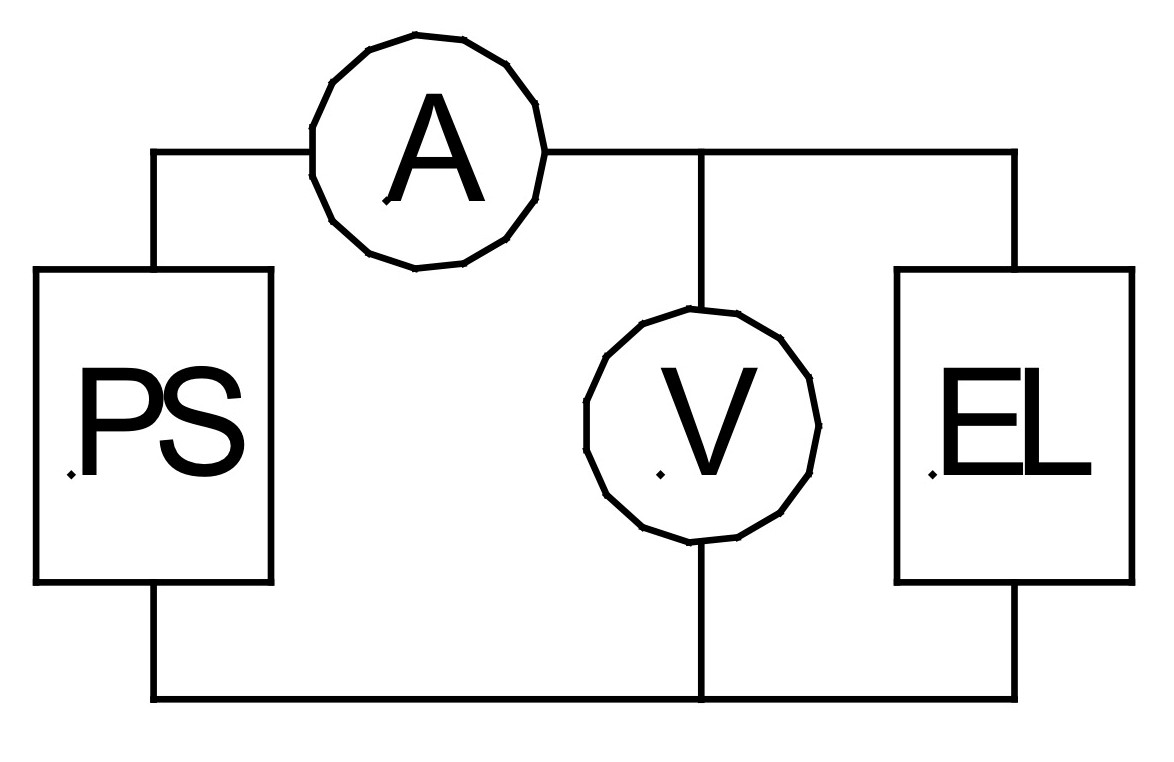
\includegraphics[width=0.4\textwidth]{../Images/l1_PartB.jpg}
\caption{\label{figB}Electrical circuit for measuring Electrolyzer input voltage and current.}
\end{figure}

An electrolyzer was supplied distilled water and electricity to produce a
given quantity of Hydrogen gas, where the current and voltage were measured
via the circuit given in \ref{figB}. The amount of time to produce a 
target amount of Hydrogen was measured, with the total energy drawn by the 
circuit and the total chemical energy produced by the electrolyzer compared
to compute the electrolyzer efficiency.

\subsection{Results}

\begin{equation}
PV = \frac{nRT}{m}
    \label{pvnrt}
\end{equation}
Where P is pressure, V is volume, n is the number of molecules, R is a constant, T is temperature, and m is mass.\\

\begin{equation}
	E_{H_2} = m_{H_2} \times HHV
    \label{HHV}
\end{equation}
Where E is energy, m is mass, and HHV is Higher Heat Value. \\

The total time to produce $5\ cm^3$ of Hydrogen gas was found to be 112
seconds, at constant voltage and current of 1.892 V and 0.3215 A. Multiplying
these quantities E = PIT, the energy consumed was found to be 68.4 joules. 
The mass of the Hydrogen was calculated using \ref{pvnrt}, assuming ideal
conditions, and the chemical energy was estimated by multiplying by the accepted
value for the Higher Heat Value of hydrogen, 141.9 MJ/kg \ref{HHV}. With a mass
of $ 4.19 \cdot 10^{-7} kg$, the stored chemical energy was found to be 59 
joules via \ref{HHV}. Finally, the efficiency of the electrolyzer was found by
\ref{eta_EL} to be $87\ \pm\ 6\%$. 

\begin{equation}
    \mathlarger{\eta}_{EL}=E_{Hydrogen}/E_E
    \label{eta_EL}
\end{equation}

\subsection{Conclusions}

This efficiency is higher than usual industrial values for electrolyzer 
efficiency given by \cite{Electrolyzer}. Assuming this particular electrolyzer
is not more efficient than most, this error most likely stems from several
measurements related to the volume of gas. Specifically:
\begin{itemize}
	\item 
		The graduations on the reservior are 1 $cm^3$, which is 1/5 the 
		total volume we were measuring.
	\item 
		The volume is used to trigger the timer, where discerning the 
		exact point the marking is reached is difficult.
\end{itemize}


\section{Hydrogen Fuel Cell}

\subsection{Procedure}

\begin{figure}[h]
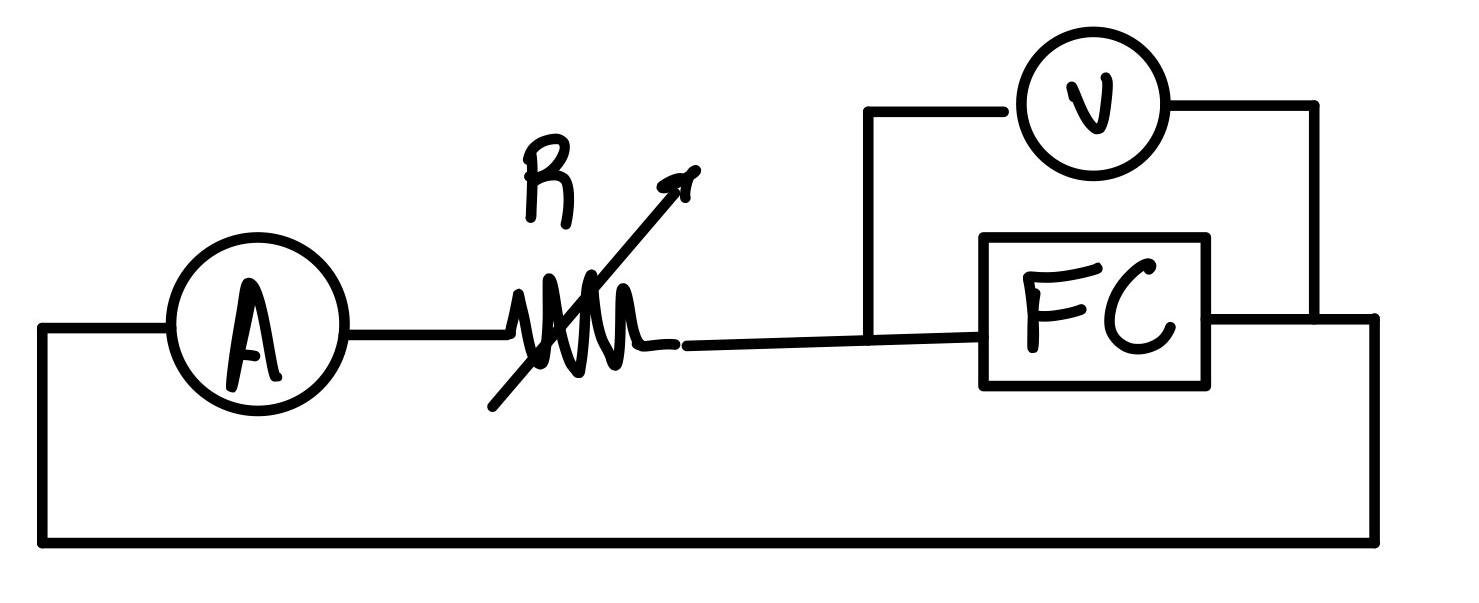
\includegraphics[width=0.4\textwidth]{../Images/l1_PartD.jpg}
\caption{\label{figD}Electrical circuit for measuring Fuel Cell output voltage and current.}
\end{figure}

A hydrogen fuel cell was supplied with hydrogen gas, in order to power a circuit
given by \ref{figD}. In the first stage of this phase of the experiment, an 
optimal resistance was found by varying R using a decade resistor,
so as to match the internal resistance of the Fuel Cell. \\

The second stage of this phase of the experiment was to then use this optimal
resistance, and a few values on either side of it, to find how much electrical
energy was produced by consuming a given quantity of hydrogen gas. The
quantity of gas and the electrical power output over time were then compared to 
compute the efficiency of the Fuel Cell.

\subsection{Results}

\begin{figure}[h]
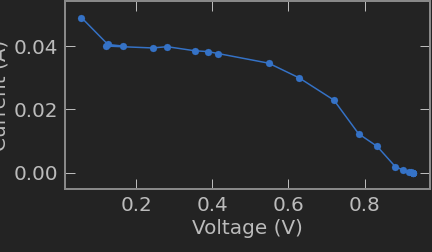
\includegraphics[width=0.45\textwidth]{../Images/l1_d_1_trial_b.png}
\caption{\label{I(V)D}Current as a function of Voltage as resistance was varied.}
\end{figure}

\begin{figure}[h]
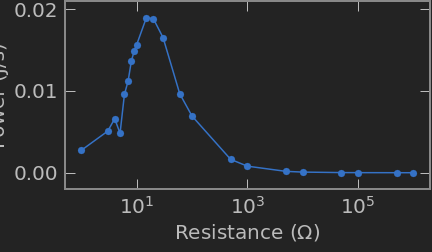
\includegraphics[width=0.45\textwidth]{../Images/l1_d_2_trial_b.png}
\caption{\label{P(R)D}Power response of the circuit at various resistances.}
\end{figure}

The optimal resistance in terms of the power response of the circuit
was found to be $15\ \Omega$ given the curve in fig. \ref{P(R)D}, 
however there was a 
delay after changing the resistance for the system to respond in terms of
output power, which resulted in a difference between the optimal resistance
computed in this stage and the optimal resistance computed at a later stage.\\

\begin{figure}[h]
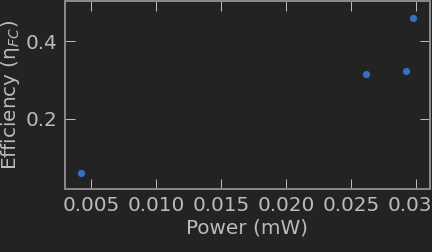
\includegraphics[width=0.45\textwidth]{../Images/l1_d_3.png}
\caption{\label{FC_n}Fuel Cell efficiency at several input powers, with varying resistance.}
\end{figure}

In the next stage of this phase of the experiment, different resistances were
used to convert what was intended to be a single given quantity of hydrogen gas 
into electrical energy. However, due to time constraints some configurations of
the circuit were only timed to consume 3 $cm^3$ of hydrogen gas, instead of 5.\\

The quantity of gas consumed was converted to mass using \ref{pvnrt}, assuming
ideal conditions. This mass was then converted into energy using the accepted
Lower Heat Value of hydrogen as given by \ref{HHV}. The electrical energy 
measured by E = tIV was then compared with the chemical energy in the hydrogen 
by \ref{eta_FC}, and plotted in \ref{FC_n}.

\begin{equation}
    \mathlarger{\eta}_{FC}=E_{FC}/E_{Hydrogen}
    \label{eta_FC}
\end{equation}

The peak efficiency was found to be $49\ \pm\ 5$.

\subsection{Conclusions}

This efficiency is much lower than the accepted value given by \cite{Fuel Cell}.
As with the Electrolyzer experiment, the uncertainty in this experiment was in 
large part due to the graduations on the gas reservior. Another likely source of
error is also our ability to find the optimal parameters for the circuit w.r.t 
the Resistance. Given the calculated values for Power and Time, it is
likely an optimal resistance would have been between 9 and 10 Ohms. Where
the capability of the decade resistor only allows resistances in steps of 1 Ohm,
and the difference between 9 and 10 Ohms meant a very small change in power but 
a large change in the time required to consume a given quantity of hydrogen gas,
it is clear we did not measure the Fuel Cell capability under ideal conditions.


\section{Summary}

The efficiency of converting various forms of energy to and from 
electrical energy were experimentally measured. \\
The efficiency of a
Silicon-based Solar Cell was found to be $15\ \pm\ 2\ \%$, in agreement
with typical performance, albeit lower than usual. The main source of error
was the spread of intensity across the solar cell, which could be improved
in future experiments.\\

The efficiency of an Electrolyzer was found to
be $87\ \pm\ 6\ \%$, which is higher than typical performance. The most 
significant source of uncertainty in this and the Hydrogen Fuel Cell experiment
stemmed from the graduations on the gas reservior, especially because there
are two measurements that stem from it. In all likeliness these errors may 
cancel, but error propogation was not handled in that way. It may be that this
value was higher because of the difference between lab conditions and standard
conditions, resulting in lower density of gas and overpredicting of the mass 
produced. \\

The efficiency of a Hydrogen Fuel Cell was found to be $49\ \pm\ 5\ \%$,
which is lower than typical performance. This again was likely in large part
due to the graduations on the gas reservior, but also could be due to a 
limitation in our ability to optimize the circuit w.r.t. resistance. 
However, the same difference between ideal conditions and lab conditions 
leading to a high result would lead to a low measured efficiency in this 
experiment, as less gas would be actually being consumed than expected and as 
such the cell was actually using less energy than measured.


\begin{widetext}
\begin{center}
\begin{table}[h]
\renewcommand{\arraystretch}{1.35}
\setlength{\tabcolsep}{10pt}
\caption{\label{}Measured and accepted values of the speed of light and refractive index of various materials.}
\begin{tabular}{|c|c|c|c|c|}
%\hline
\toprule
Apparatus &  $\eta$ (\%) & Accepted $\eta$ value & Refs. & Deviation \\
\colrule
Photovoltaic Cell &  $15 \pm 2$ & $17 \pm 2.5$ & \cite{Solar Cell} & $0\sigma$  \\
\colrule
Elecrolyzer &  $87 \pm 6$ & 80 & \cite{Electrolyzer} & $2\sigma$  \\
\colrule
Hydrogen Fuel Cell &  $49 \pm 5$ & 60 & \cite{Fuel Cell} & $-3\sigma$  \\
%\hline
\botrule
\end{tabular}
\end{table}
\end{center}
\end{widetext}





\begin{thebibliography}{9}
%
\bibitem{HHV} 
Wikipedia, Heat of Combustion: \\
\href{https://en.wikipedia.org/wiki/Heat_of_combustion}{https://www.wikepedia.com}
%
\bibitem{Solar Cell} 
Energysage, Most Efficient Solar Panels\\
\href{https://news.energysage.com/what-are-the-most-efficient-solar-panels-on-the-market/#:~:text=How%20efficient%20are%20solar%20panels,are%20not%20above%2020%25%20efficiency.}{https://www.energysage.com/}
%
\bibitem{Electrolyzer} 
Carbon Commentary, Hydrogen made by Electolysis\\
\href{https://www.carboncommentary.com/blog/2017/7/5/hydrogen-made-by-the-electrolysis-of-water-is-now-cost-competitive-and-gives-us-another-building-block-for-the-low-carbon-economy}{https://www.carboncommentary.com}
%

%
\bibitem{Fuel Cell} 
Energy.gov, Fuel Cell Fact Sheet\\
\href{https://www.energy.gov/sites/prod/files/2015/11/f27/fcto_fuel_cells_fact_sheet.pdf}{https://www.energy.gov}

\end{thebibliography}


\end{document}
%
% ****** End of file apstemplate.tex ******

